\documentclass[14pt]{extreport}
\usepackage{cmap}
\usepackage[utf8]{inputenc}
\usepackage[english,ukrainian]{babel}
\usepackage{graphicx}
\usepackage{geometry}
\usepackage{listings}
\usepackage{amsmath}
\usepackage{float}
\usepackage{array}
\geometry{
	a4paper,
	left=20mm,
	right=20mm,
	top=20mm,
	bottom=20mm
}
\lstset{
	language=bash,
	tabsize=4,
	breaklines,
	keepspaces,
	showstringspaces=false,
}
\graphicspath{ {./pictures} }
\setlength{\parindent}{4em}

\newcommand\subject{Аналіз вимог до програмного забезпечення}
\newcommand\lecturer{професор кафедри ПЗ\\Грицюк Ю.І.}
\newcommand\teacher{асистент кафедри ПЗ\\Масюкевич В.В.}
\newcommand\mygroup{ПЗ-32}
\newcommand\lab{4}
\newcommand\theme{Засіб Tiger PRO для управління вимогами до програмного забезпечення}
\newcommand\purpose{Ознайомитися із програмним засобом управління вимогами,
	вивчити основні характеристики та можливості}

\begin{document}
\begin{normalsize}
	\begin{titlepage}
		\thispagestyle{empty}
		\begin{center}
			\textbf{МІНІСТЕРСТВО ОСВІТИ І НАУКИ УКРАЇНИ\\
				НАЦІОНАЛЬНИЙ УНІВЕРСИТЕТ "ЛЬВІВСЬКА ПОЛІТЕХНІКА"}
		\end{center}
		\begin{flushright}
			Інститут \textbf{КНІТ}\\
			Кафедра \textbf{ПЗ}
		\end{flushright}
		\vspace{140pt}
		\begin{center}
			\textbf{ЗВІТ}\\
			\vspace{10pt}
			До лабораторної роботи № \lab\\
			\textbf{На тему}: “\textit{\theme}”\\
			\textbf{З дисципліни}: “\subject”
		\end{center}
		\vspace{40pt}
		\begin{flushright}
			
			\textbf{Лектор}:\\
			\lecturer\\
			\vspace{10pt}
			\textbf{Виконав}:\\
			
			студент групи \mygroup\\
			Коваленко Д.М.\\
			\vspace{10pt}
			\textbf{Прийняв}:\\
			
			\teacher\\
			
			\vspace{28pt}
			«\rule{1cm}{0.15mm}» \rule{1.5cm}{0.15mm} 2023 р.\\
			$\sum$ = \rule{1cm}{0.15mm}……………\\
			
		\end{flushright}
		\vspace{\fill}
		\begin{center}
			\textbf{Львів — 2023}
		\end{center}
	\end{titlepage}
		
	\begin{description}
		\item[Тема.] \theme.
		\item[Мета.] \purpose.
	\end{description}

	\section*{Лабораторне завдання}
	\begin{enumerate}
		\item Внесення специфікації вимог до ПЗ в
		програмний засіб для управління вимогами.
		\item Розробити ієрархічну структуру вимог та внести специфікацію
		до програмного продукту (на задану тему) у засіб управління вимогами.
	\end{enumerate}
	
	\begin{figure}[H]
		\centering
		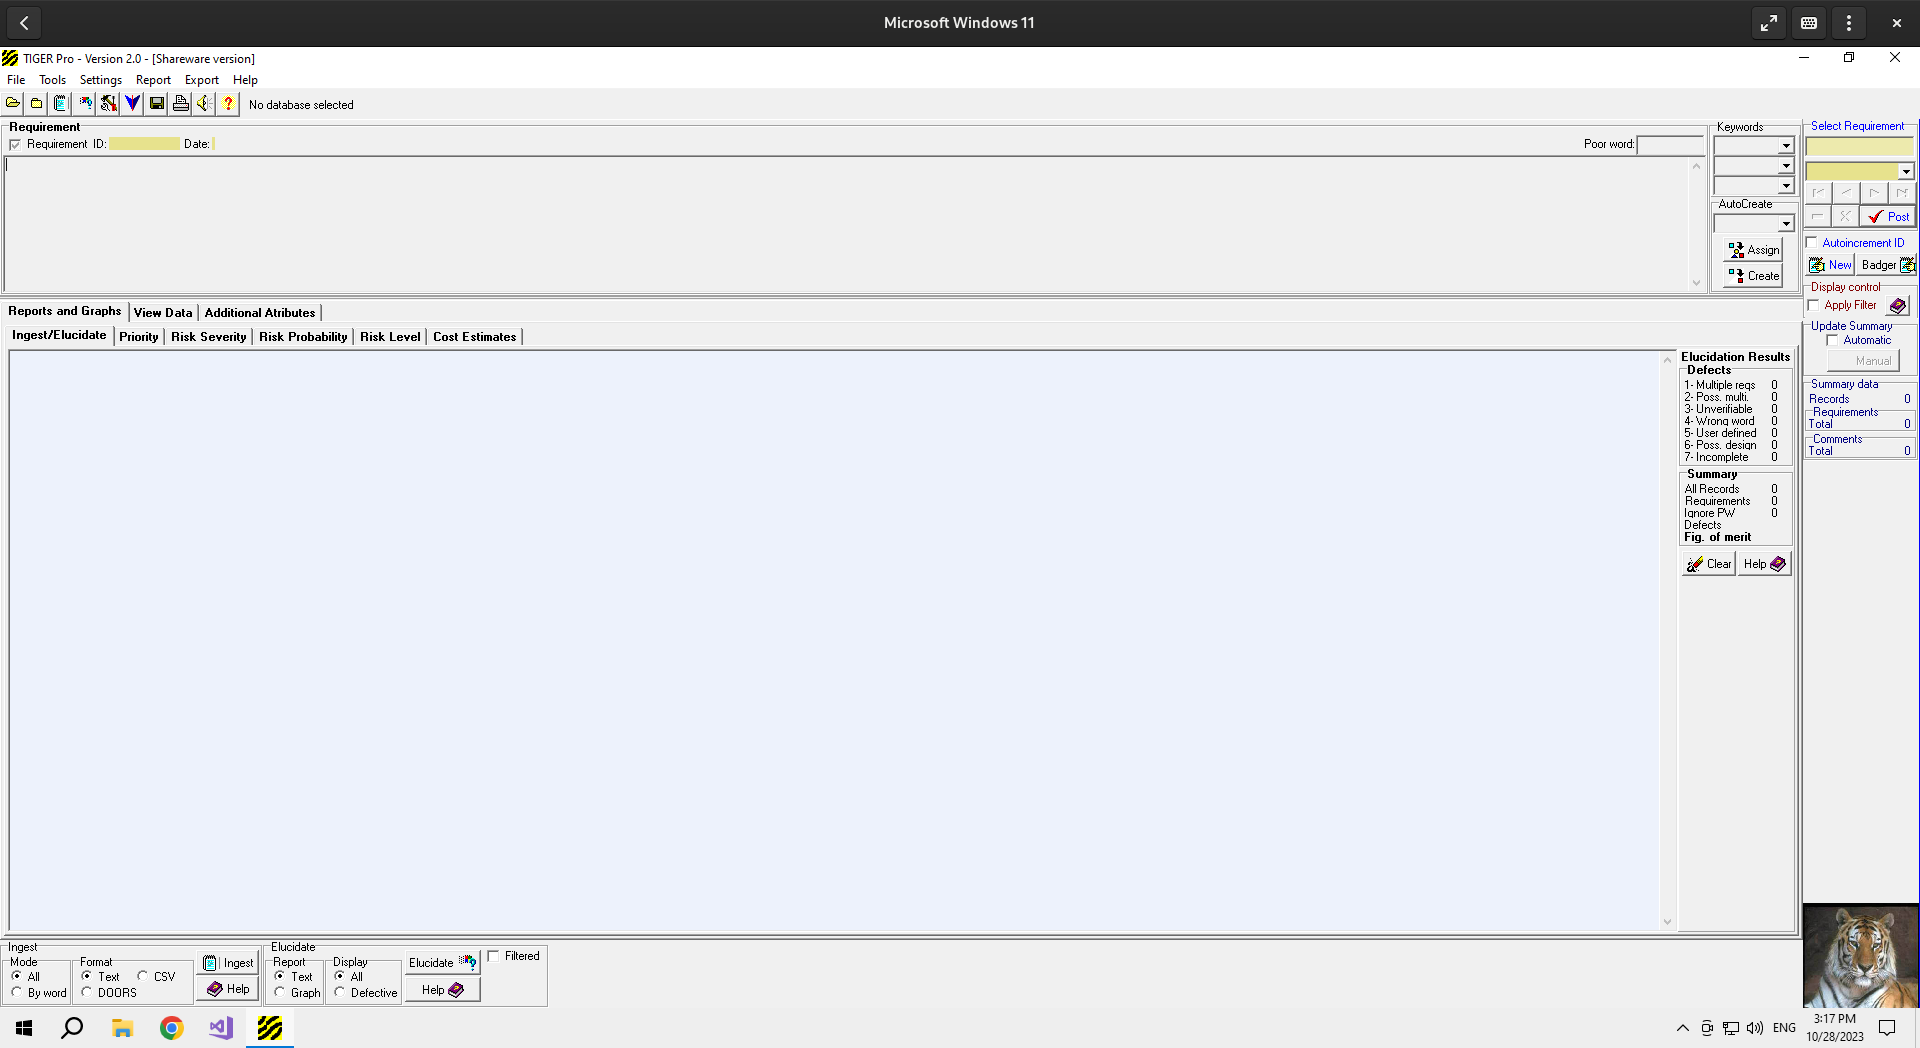
\includegraphics[scale=0.25]{1}
		\caption{Новий проект}
	\end{figure}

	\begin{figure}[H]
		\centering
		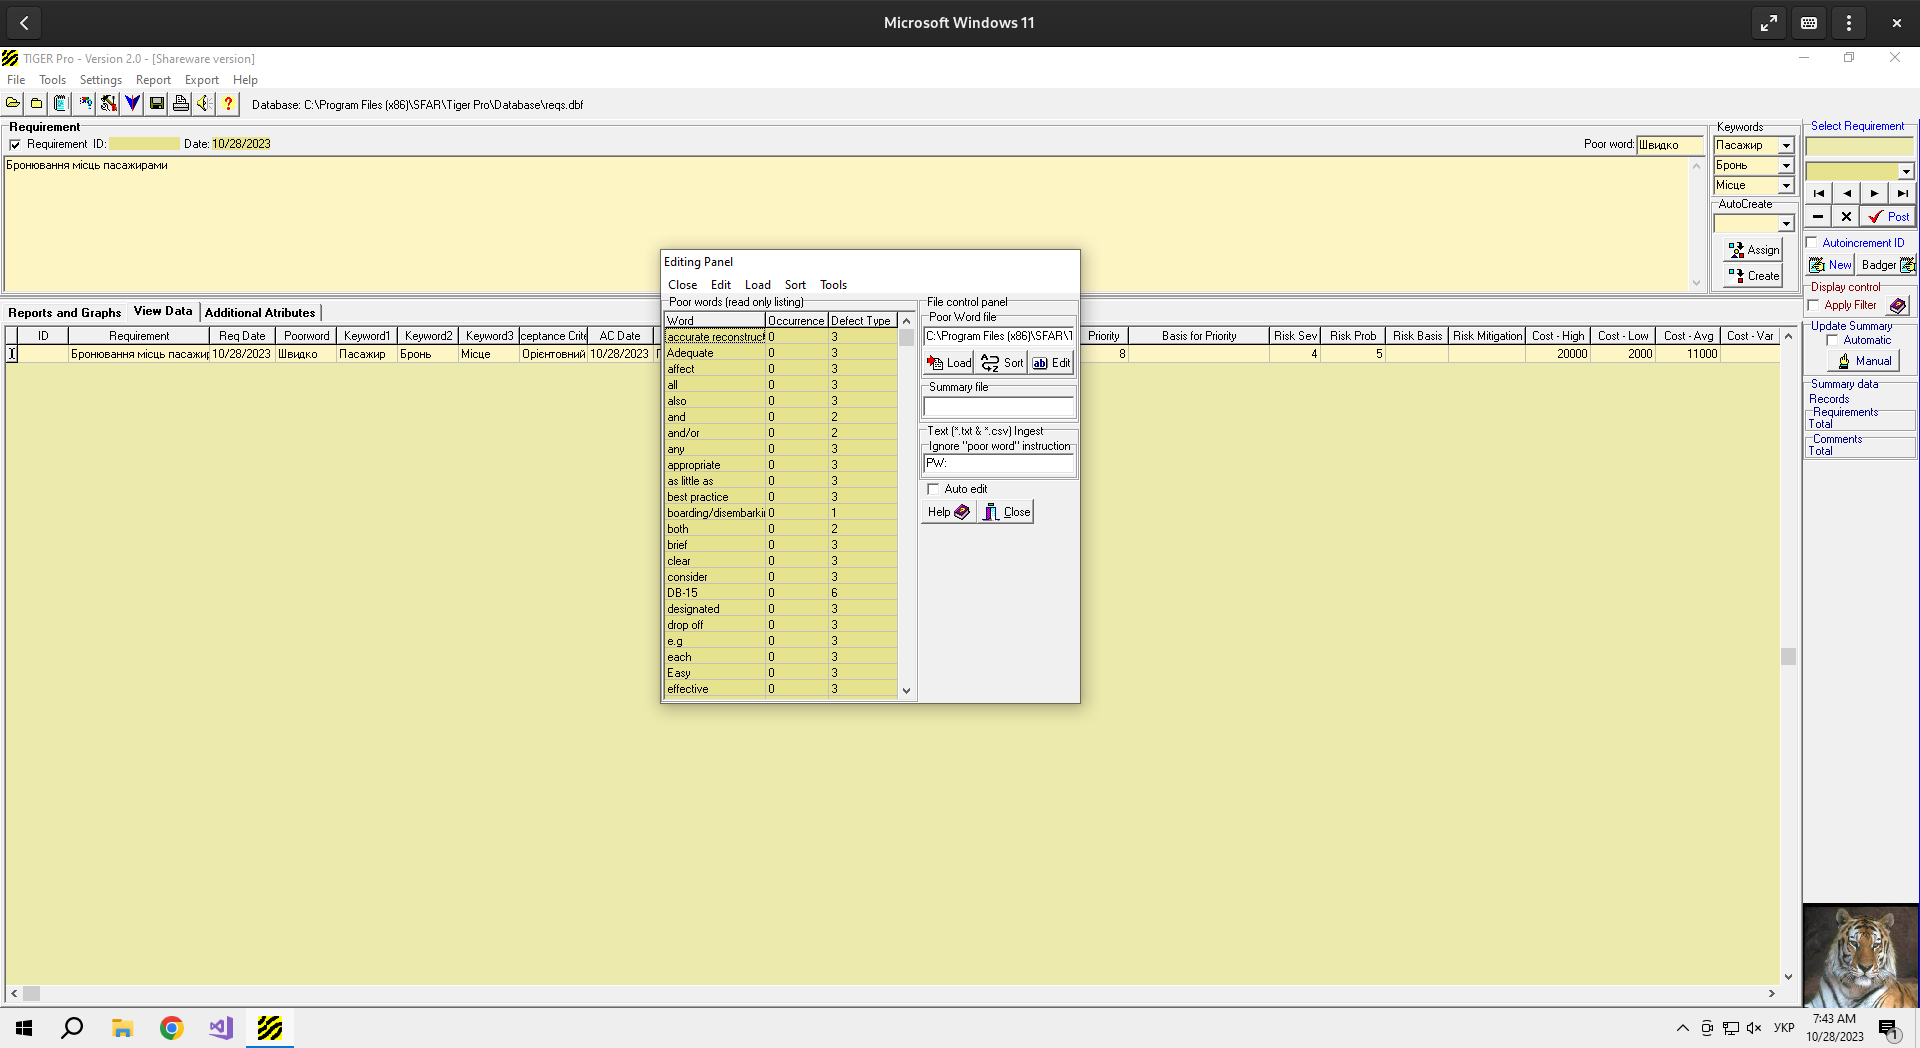
\includegraphics[scale=0.25]{2}
		\caption{Редактор хибних слів}
	\end{figure}
	
	\begin{figure}[H]
		\centering
		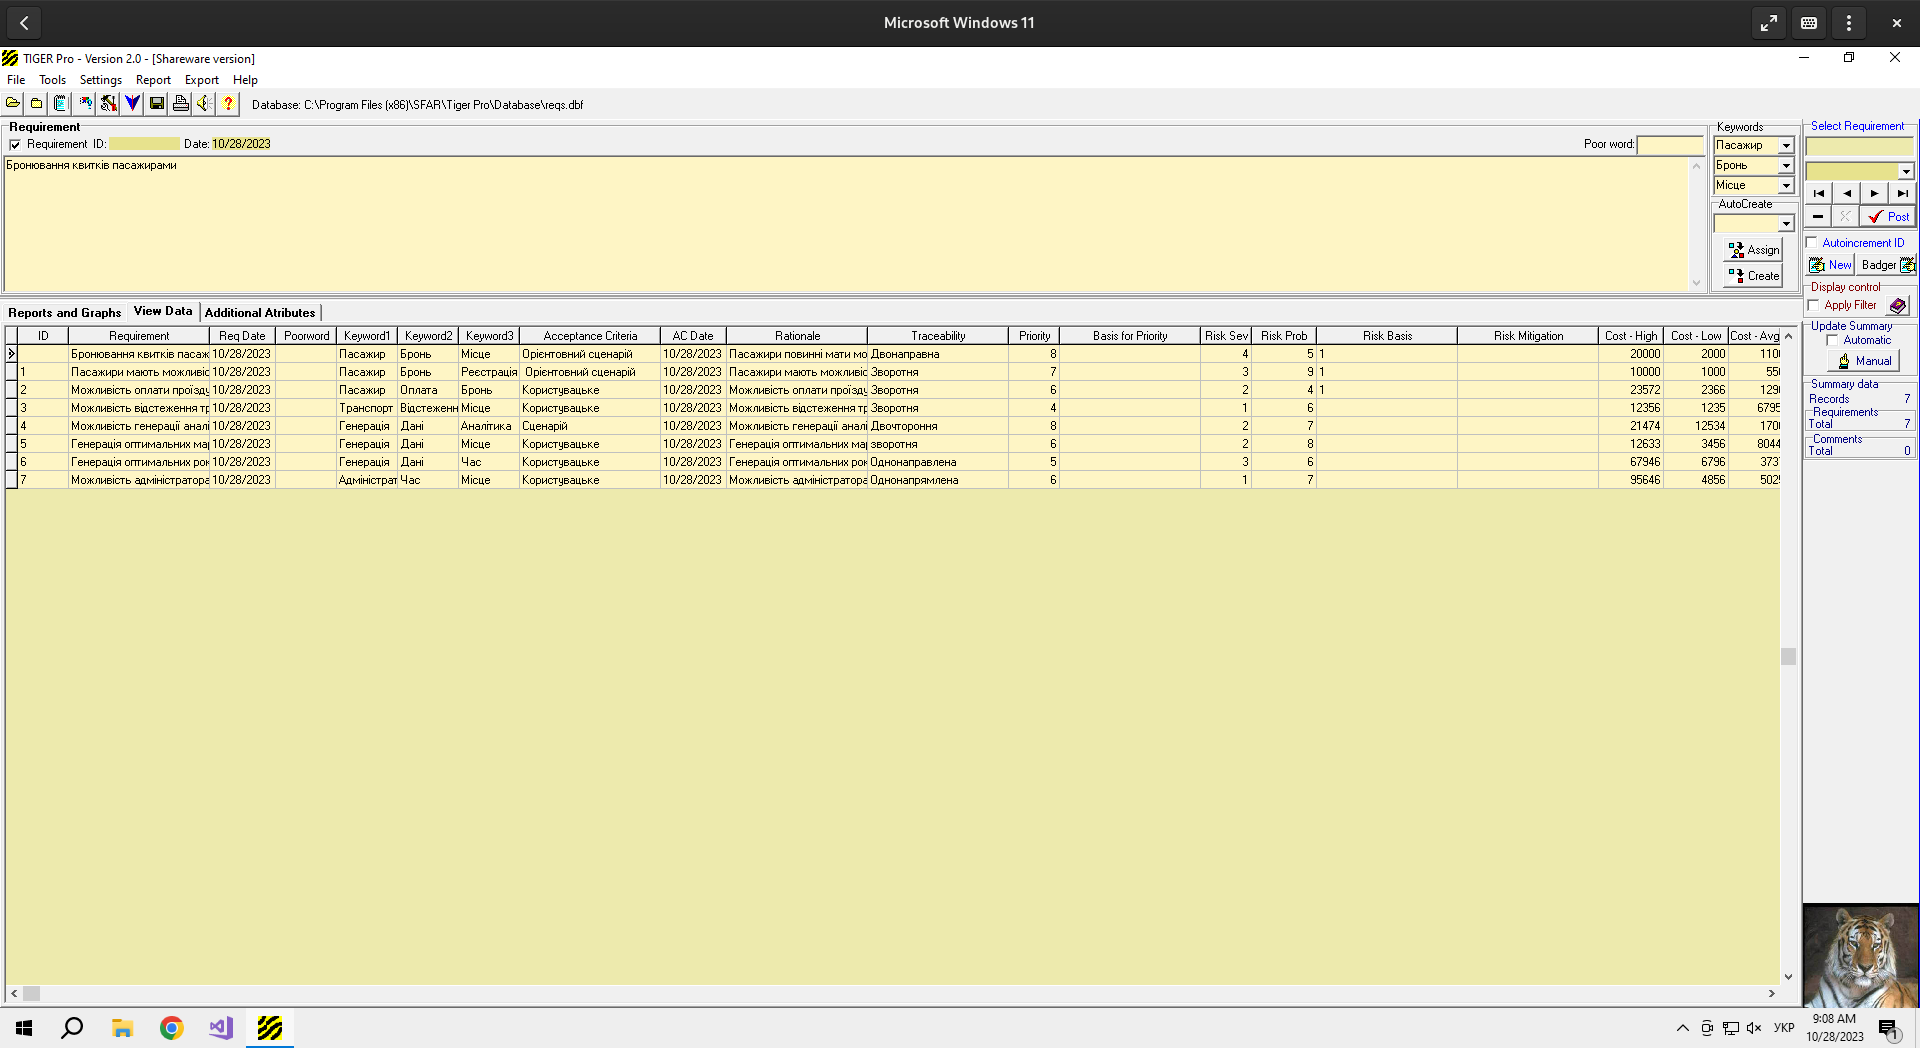
\includegraphics[scale=0.5]{3}
		\caption{Проект із внесеними вимогами}
	\end{figure}
	
	\begin{figure}[H]
		\centering
		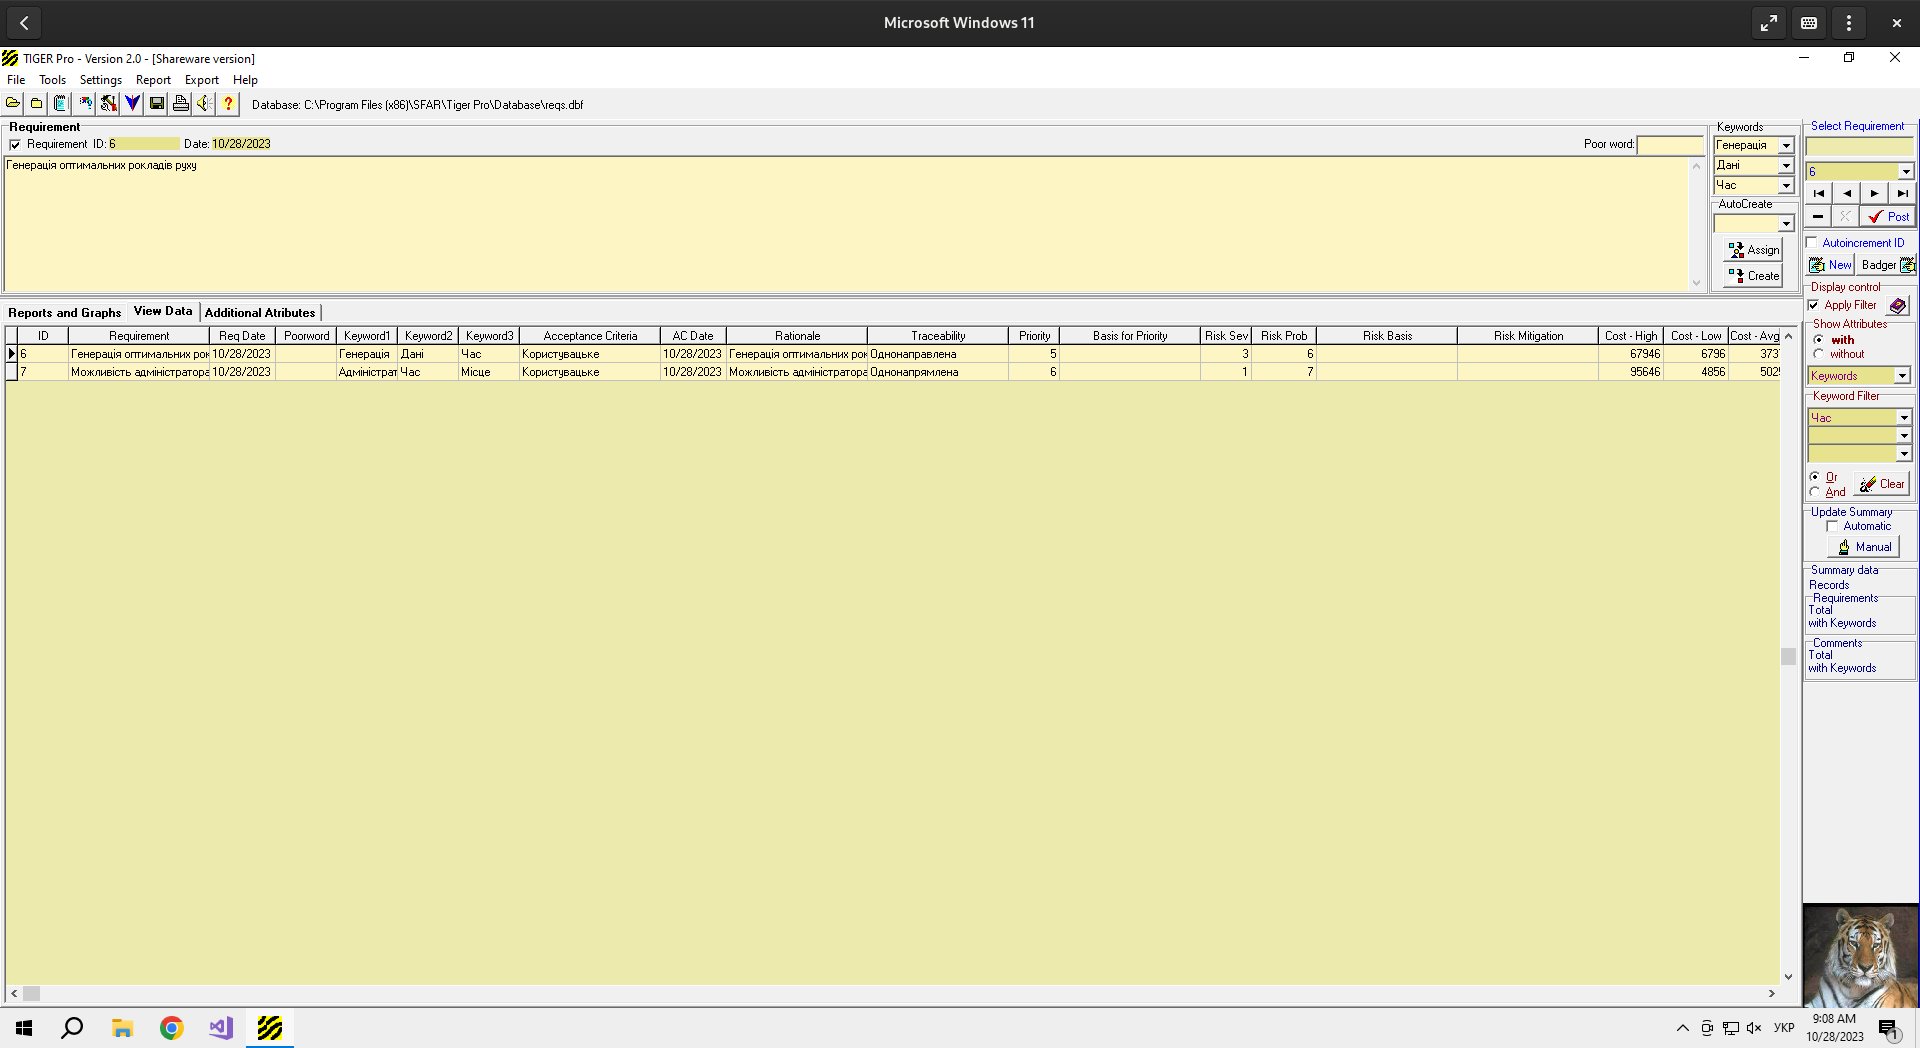
\includegraphics[scale=0.5]{4}
		\caption{Фільтрування вимог за ключовим словом}
	\end{figure}
	
	\begin{figure}[H]
		\centering
		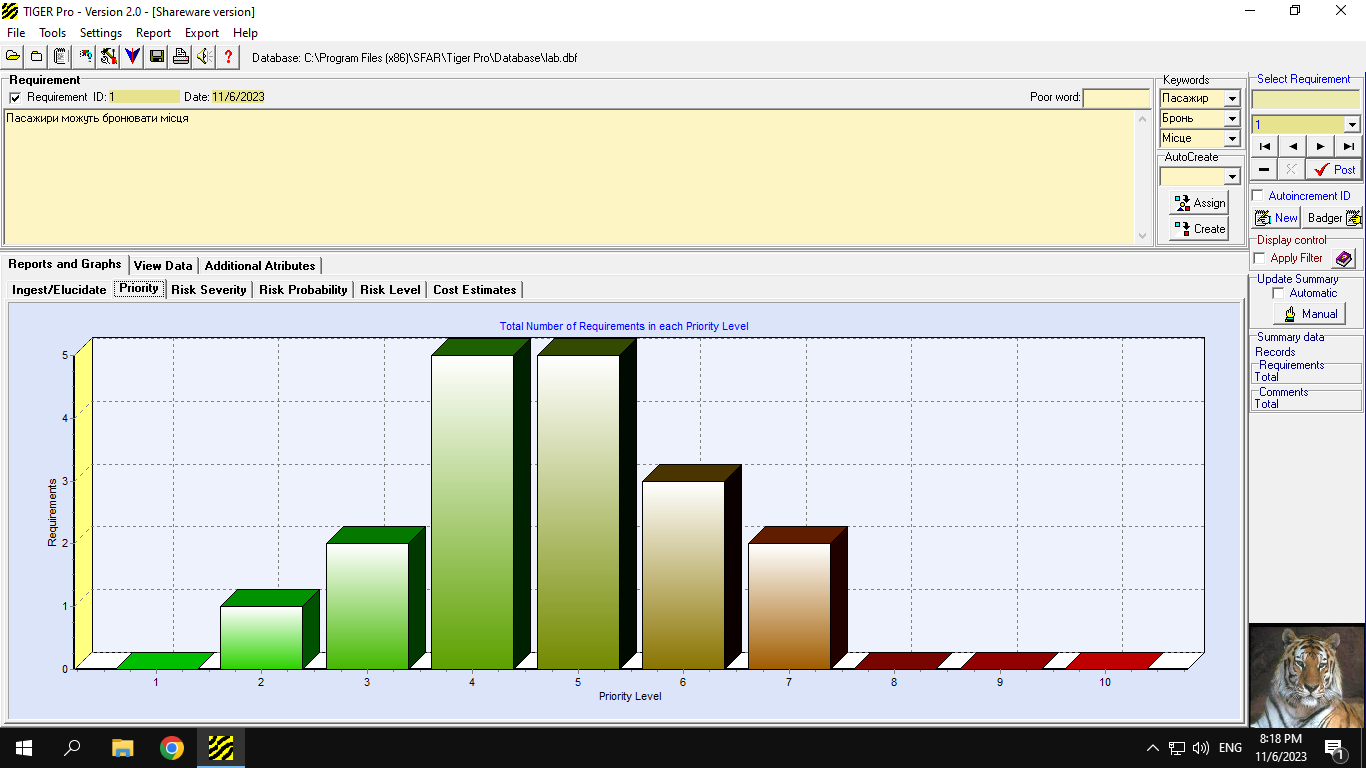
\includegraphics[scale=0.5]{5}
		\caption{Діаграма пріоритетів}
	\end{figure}
	
	\begin{figure}[H]
		\centering
		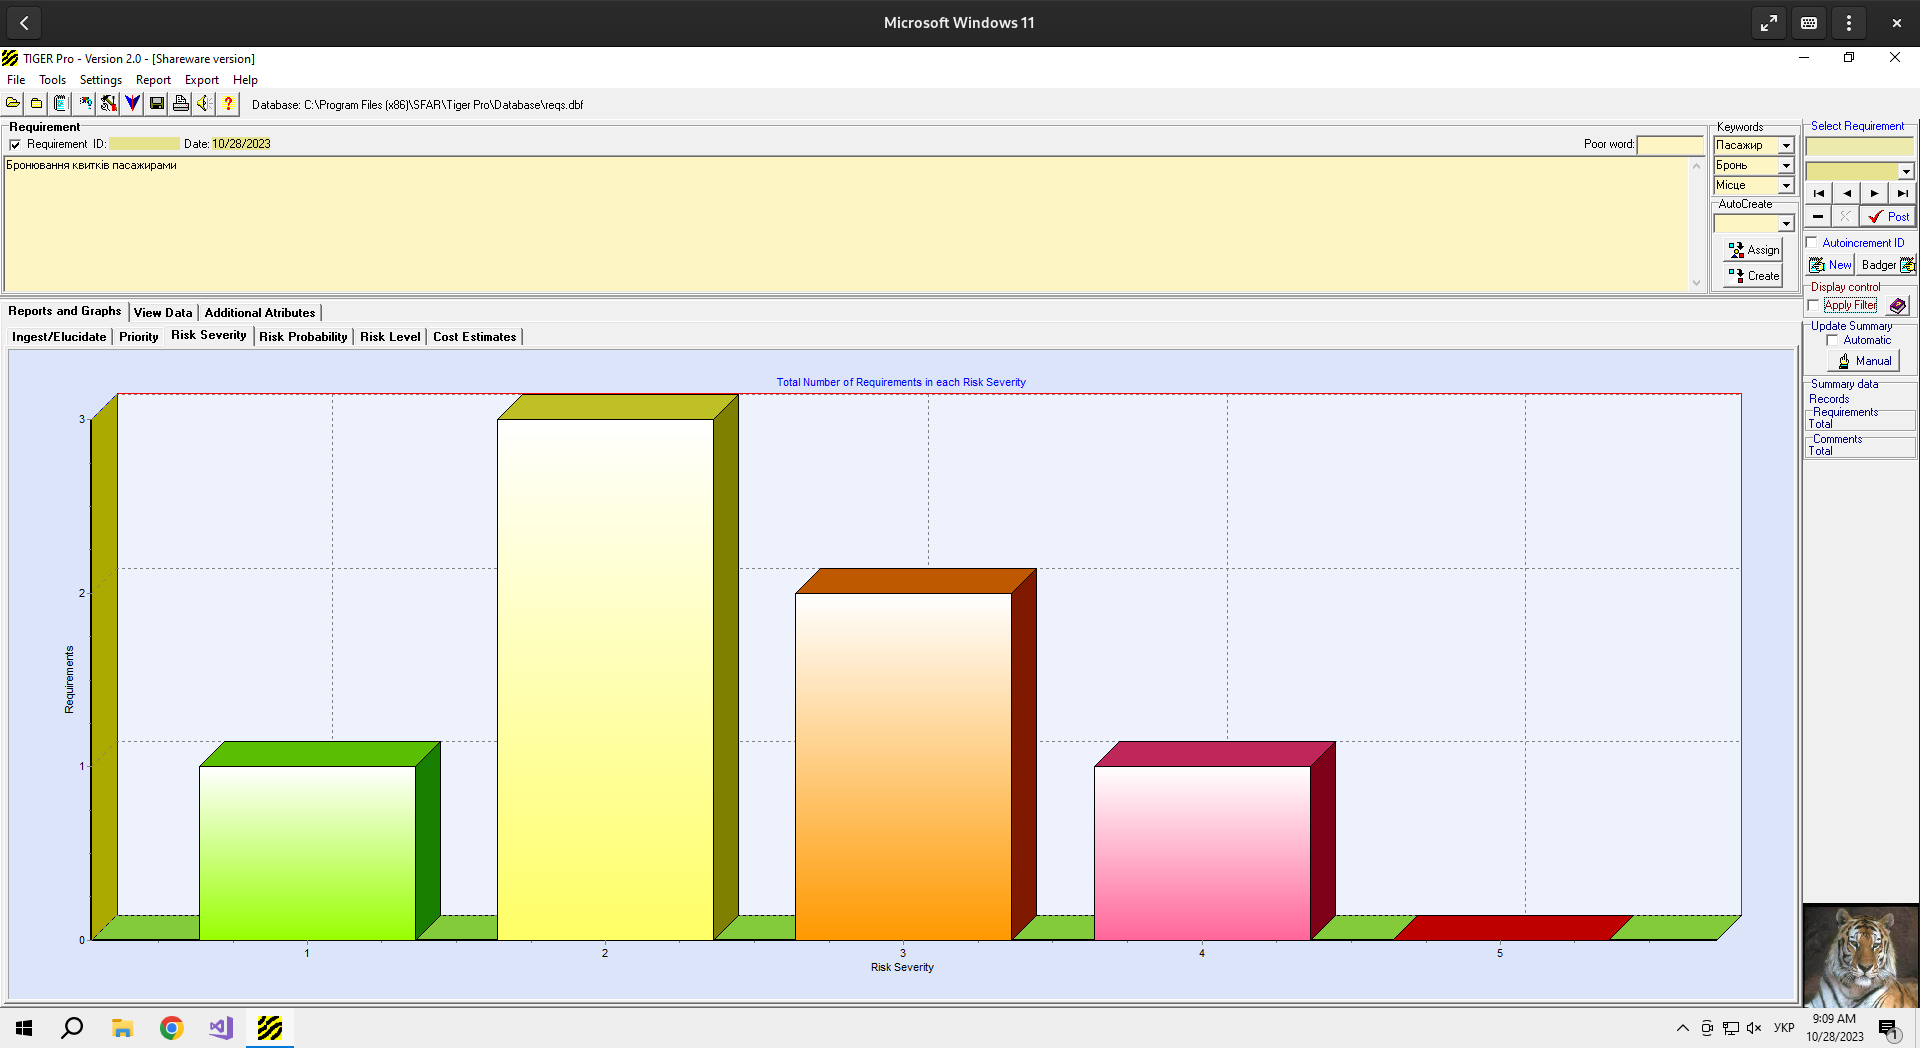
\includegraphics[scale=0.5]{6}
		\caption{Діаграма ризиків}
	\end{figure}
	
	\begin{figure}[H]
		\centering
		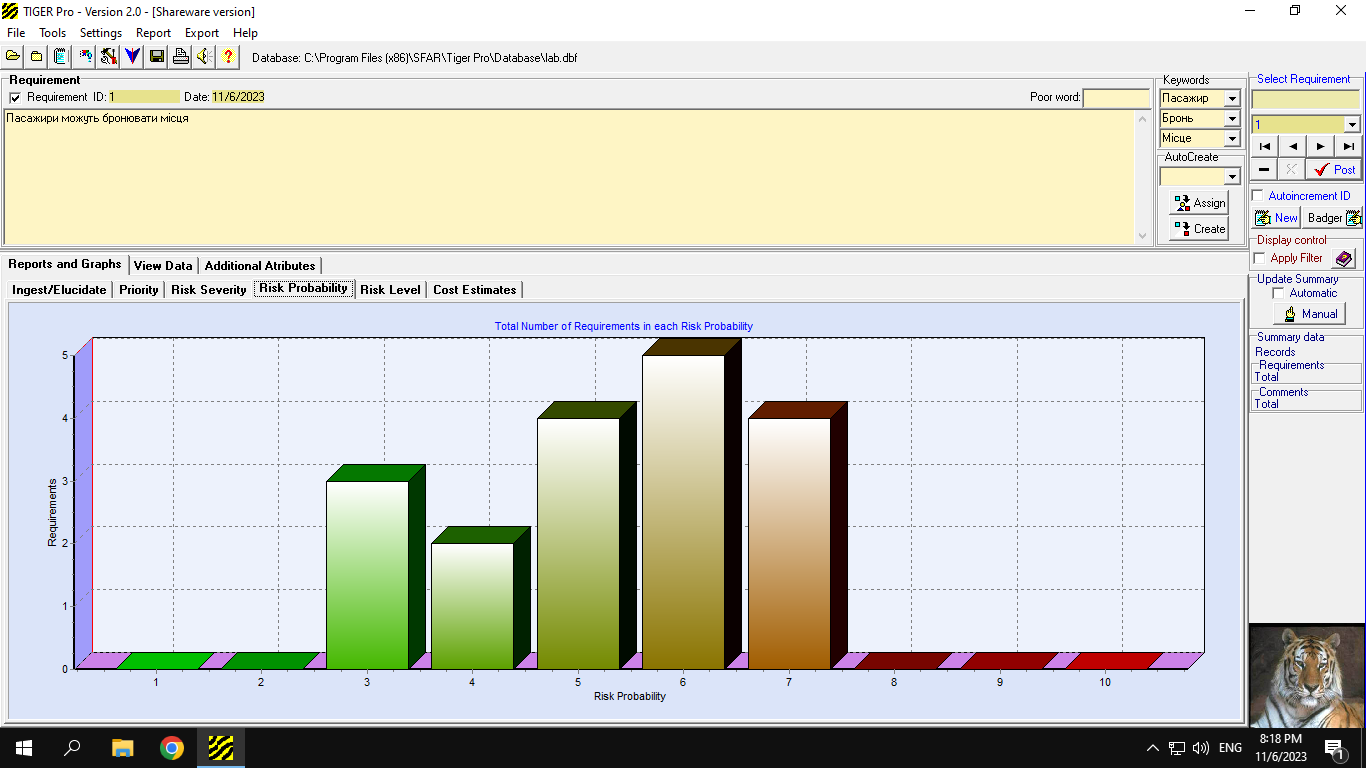
\includegraphics[scale=0.5]{7}
		\caption{Діаграма Ризиків}
	\end{figure}
	
	\begin{figure}[H]
		\centering
		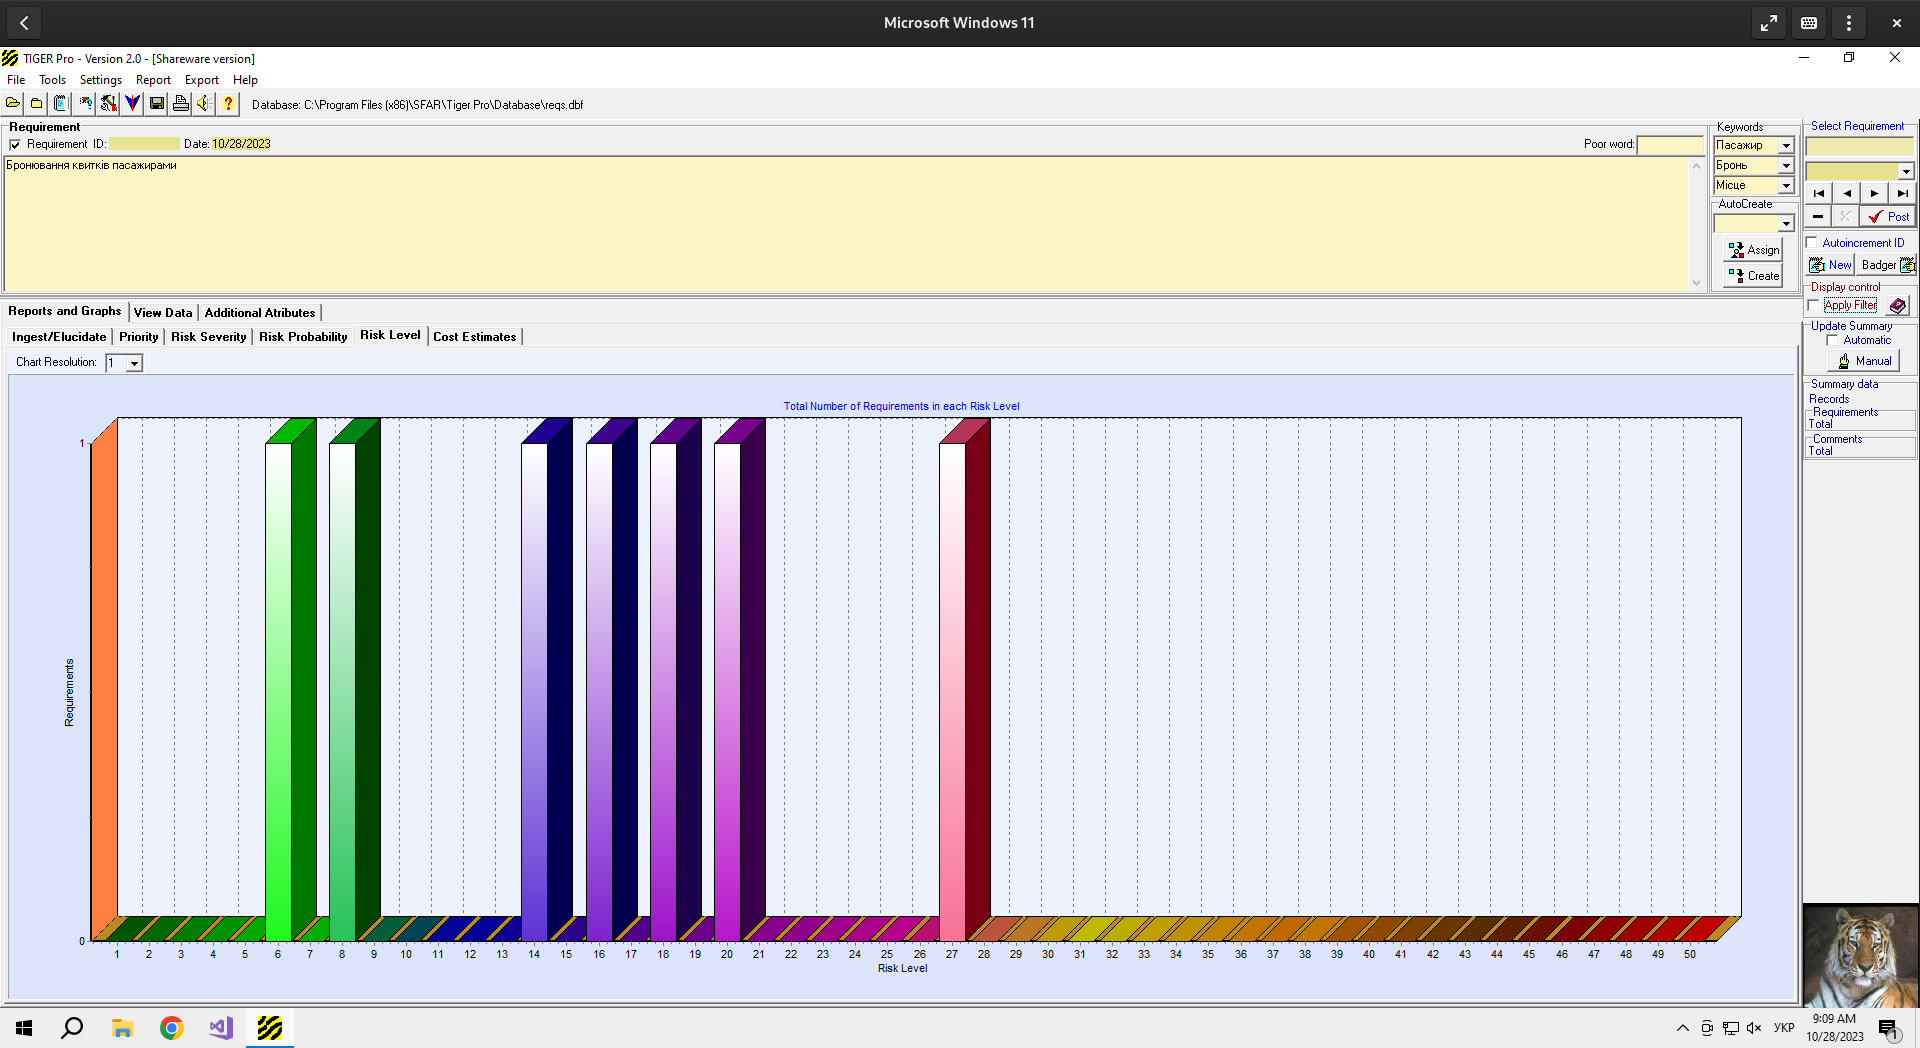
\includegraphics[scale=0.5]{8}
		\caption{Діаграма ризиків}
	\end{figure}
	
	\begin{figure}[H]
		\centering
		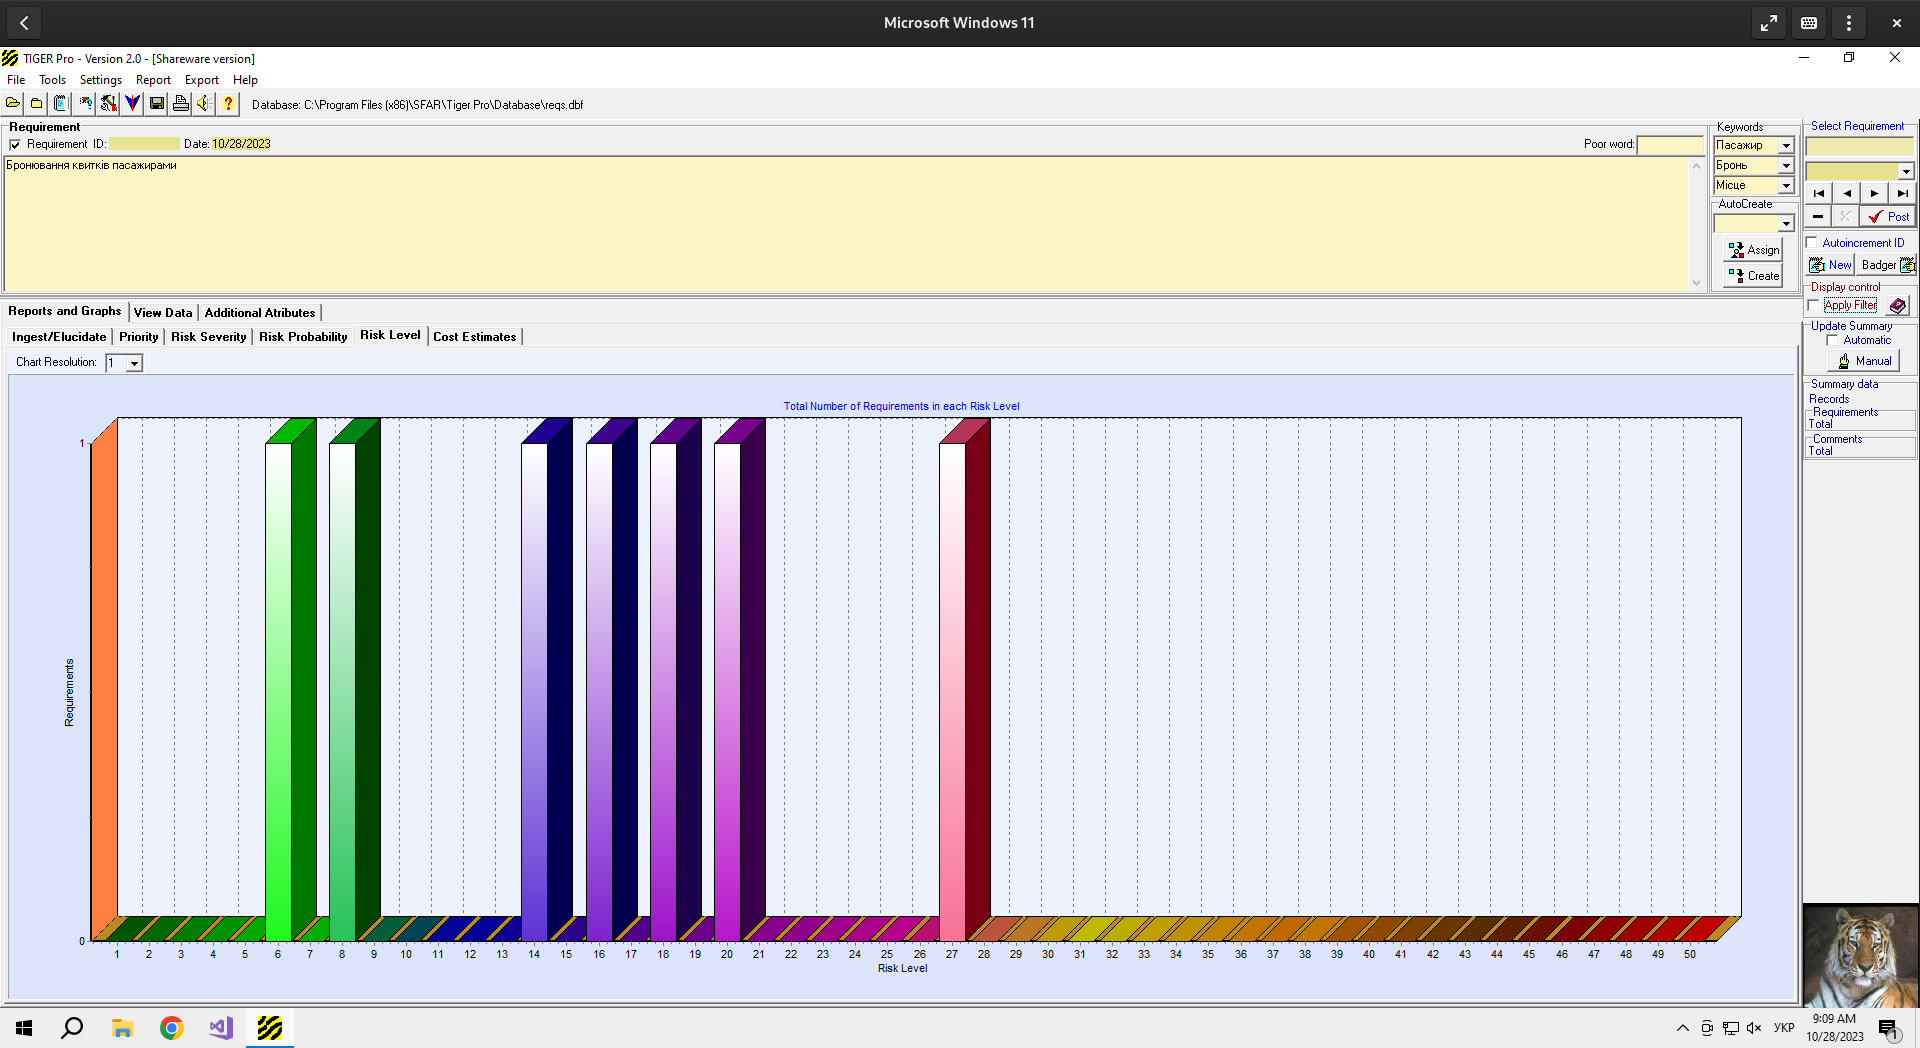
\includegraphics[scale=0.5]{8}
		\caption{Вартість}
	\end{figure}
	\section*{Висновок}
	Під час виконання лабораторної роботи я ознайомився з програмним засобом управління вимогами, вивчив основні характеристики та можливості.
	
\end{normalsize}
\end{document}
